\documentclass[tikz,border=7pt]{standalone}
\usepackage{amsmath,amssymb}
\usetikzlibrary{arrows.meta,calc,positioning,decorations.pathreplacing}

% ============================================================
% Three explicit, sphere-specialized pictures at p = (0,0,1):
%   (1) Gauss map  N:S^2->S^2,  p |-> p
%   (2) Differential (dN)_p : T_p S^2 -> T_{N(p)} S^2  with (dN)_p(v)=v
%   (3) Shape operator S_p = -(dN)_p : T_p S^2 -> T_p S^2 with S_p(v)=-v
%
% All drawings are in the xz cross-section (y=0), where:
%   S^2 ∩ {y=0} is the unit circle x^2+z^2=1,
%   p = (0,1) in this cross-section,
%   v corresponds to (1,0,0) (drawn as (1,0) in the cross-section).
% ============================================================

\begin{document}
% ============================================================
% (2) Differential (dN)_p : T_p S^2 -> T_{N(p)} S^2, and (dN)_p(v)=v
% ============================================================
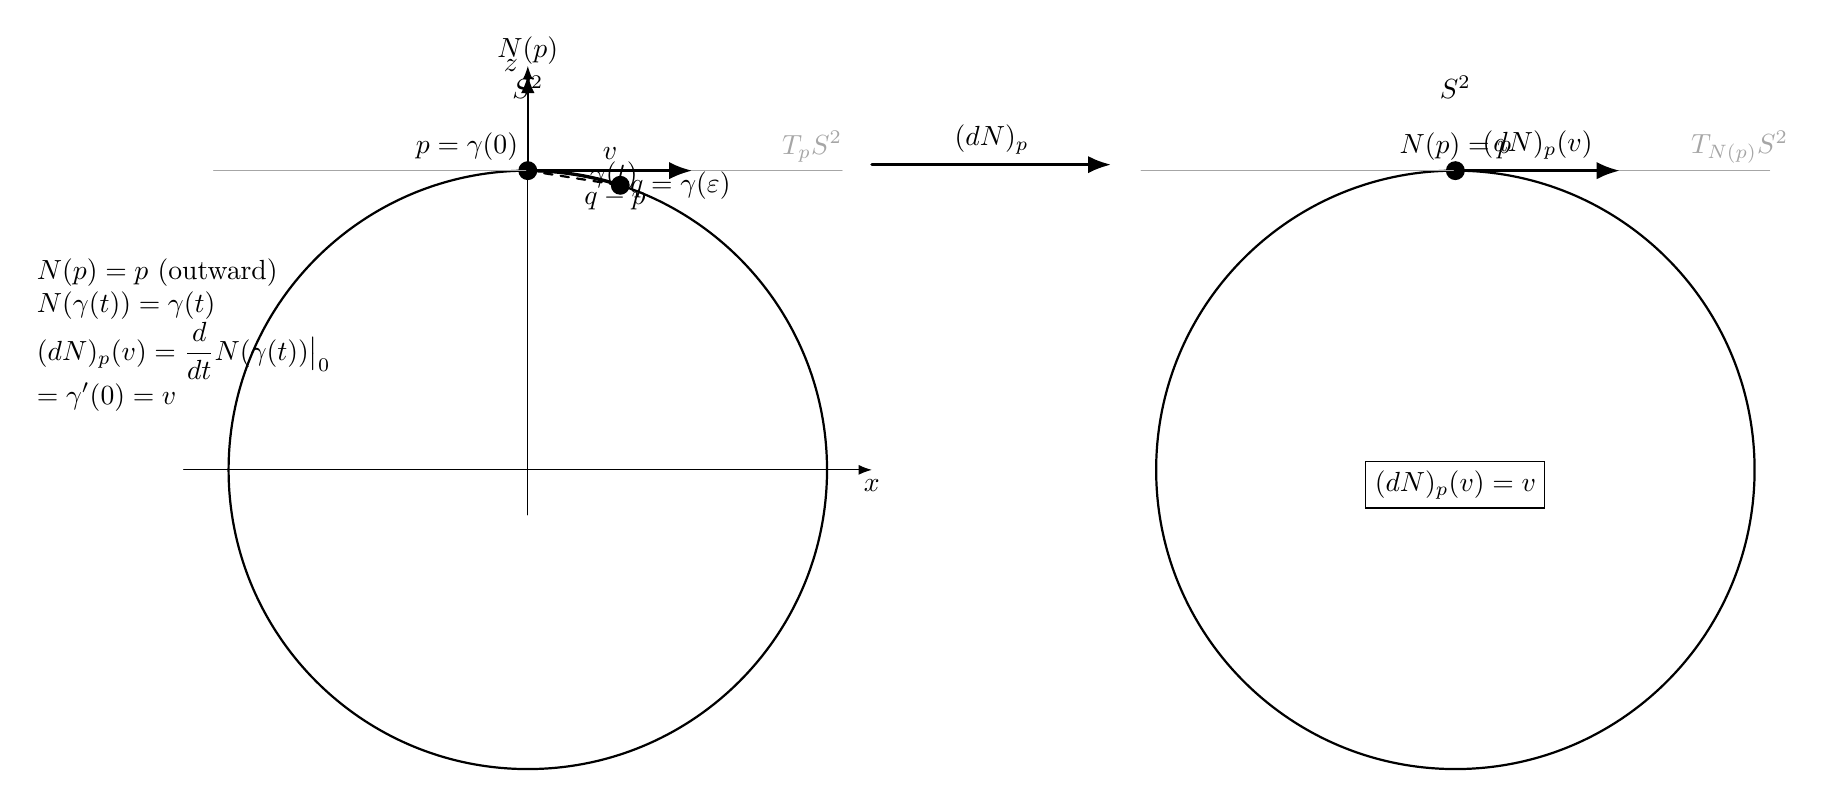
\begin{tikzpicture}[>=Latex, line cap=round, line join=round, scale=3.8]
	
	% Choose a concrete small step epsilon for a finite-difference picture
	\def\epsdeg{18}
	\pgfmathsetmacro{\sE}{sin(\epsdeg)}
	\pgfmathsetmacro{\cE}{cos(\epsdeg)}
	\pgfmathsetmacro{\epsrad}{\epsdeg*pi/180}
	
	% Left: S^2 with curve gamma(t) and v at p
	\begin{scope}[shift={(0,0)}]
		\draw[thick] (0,0) circle (1);
		\node at (0,1.28) {$S^2$};
		
		% axes
		\draw[->] (-1.15,0) -- (1.15,0) node[below] {$x$};
		\draw[->] (0,-0.15) -- (0,1.35) node[left] {$z$};
		
		% points p and q = gamma(eps)
		\coordinate (p) at (0,1);
		\coordinate (q) at (\sE,\cE);
		\fill (p) circle (0.9pt) node[above left] {$p=\gamma(0)$};
		\fill (q) circle (0.9pt) node[right] {$q=\gamma(\varepsilon)$};
		
		% curve gamma(t) = (sin t, cos t) in cross-section (y=0)
		\draw[very thick]
		(p) arc[start angle=90, end angle=90-\epsdeg, radius=1]
		node[pos=0.55, right] {$\gamma(t)$};
		
		% tangent line at p (horizontal)
		\draw[gray!70] (-1.05,1) -- (1.05,1);
		\node[gray!70] at (0.95,1.08) {$T_pS^2$};
		
		% tangent vector v = gamma'(0) = (1,0,0)  (drawn as (1,0) in cross-section)
		\draw[very thick,->] (p) -- ++(0.55,0) node[midway, above] {$v$};
		
		% normal at p : N(p)=p
		\draw[thick,->] (p) -- ++(0,0.32) node[above] {$N(p)$};
		
		% chord q-p for finite difference N(q)-N(p)=q-p (since N=Id)
		\draw[thick,dashed] (p) -- (q) node[midway, below right] {$q-p$};
		
		% label the finite difference quotient (schematic)
		\node[align=left] at (-1.15,0.45) {%
			$\displaystyle N(p)=p$ (outward)\\
			$\displaystyle N(\gamma(t))=\gamma(t)$\\
			$\displaystyle (dN)_p(v)=\frac{d}{dt}N(\gamma(t))\big|_{0}$\\
			$\displaystyle =\gamma'(0)=v$};
	\end{scope}
	
	% Right: Codomain tangent space at N(p)=p (same plane)
	\begin{scope}[shift={(3.1,0)}]
		\draw[thick] (0,0) circle (1);
		\node at (0,1.28) {$S^2$};
		
		% point N(p)=p at top
		\coordinate (np) at (0,1);
		\fill (np) circle (0.9pt) node[above] {$N(p)=p$};
		
		% tangent line at N(p) (horizontal)
		\draw[gray!70] (-1.05,1) -- (1.05,1);
		\node[gray!70] at (0.95,1.08) {$T_{N(p)}S^2$};
		
		% show (dN)_p(v) = v
		\draw[very thick,->] (np) -- ++(0.55,0) node[midway, above] {$(dN)_p(v)$};
		\node[align=center] at (0,-0.05) {$\boxed{(dN)_p(v)=v}$};
	\end{scope}
	
	% arrow indicating the differential map
	\draw[very thick,->] (1.15,1.02) -- (1.95,1.02) node[midway, above] {$(dN)_p$};
	
\end{tikzpicture}	
\end{document}
